In questo esperimento, \'{e} stato attaccato al sensore un filo con appeso un oggetto di 0.155Kg. 
Il braccio \'{e} stato posizionato in modo tale che la forza peso gravasse solo su un asse del sensore alla volta. 
In Figura \ref{fig:setup_z}, viene mostrato il setup per l'esperimento lungo l'asse z. 
\begin{figure}[H]
    \centering
    \begin{subfigure}[b]{0.4\textwidth}
        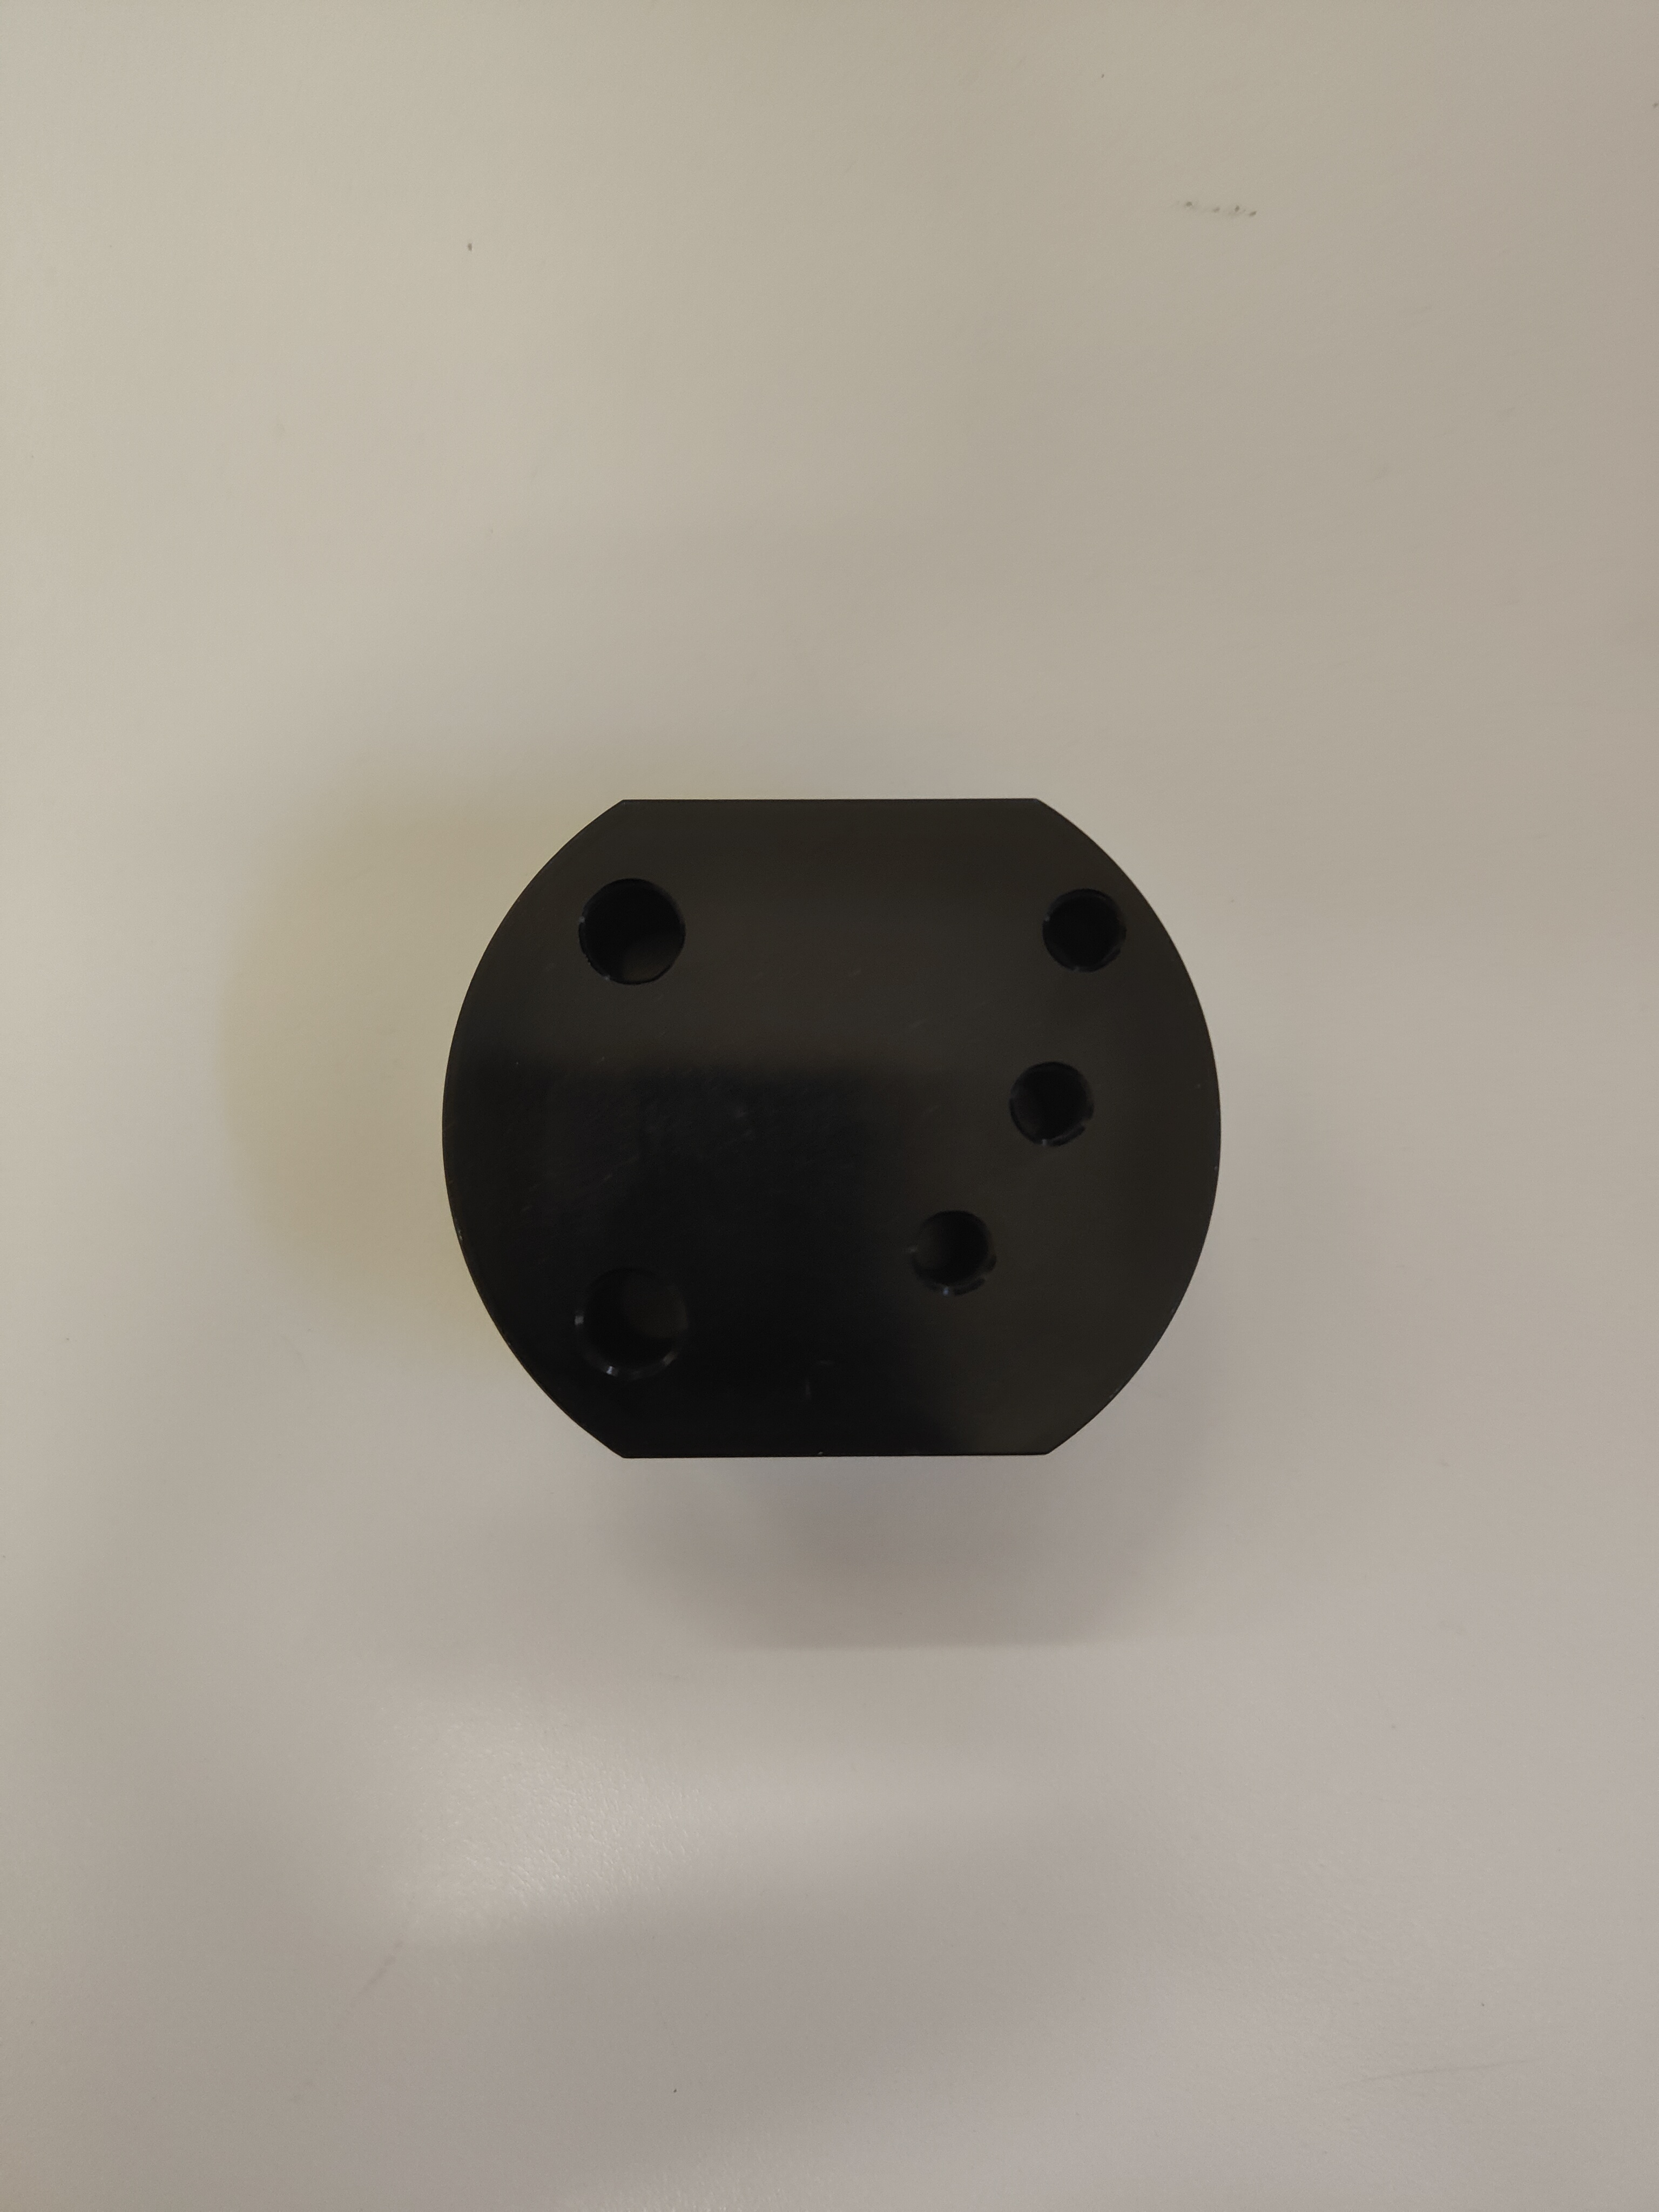
\includegraphics[width=\textwidth]{images/object.jpg}
        \label{fig:object}
    \end{subfigure}
    \qquad
    \begin{subfigure}[b]{0.4\textwidth}
        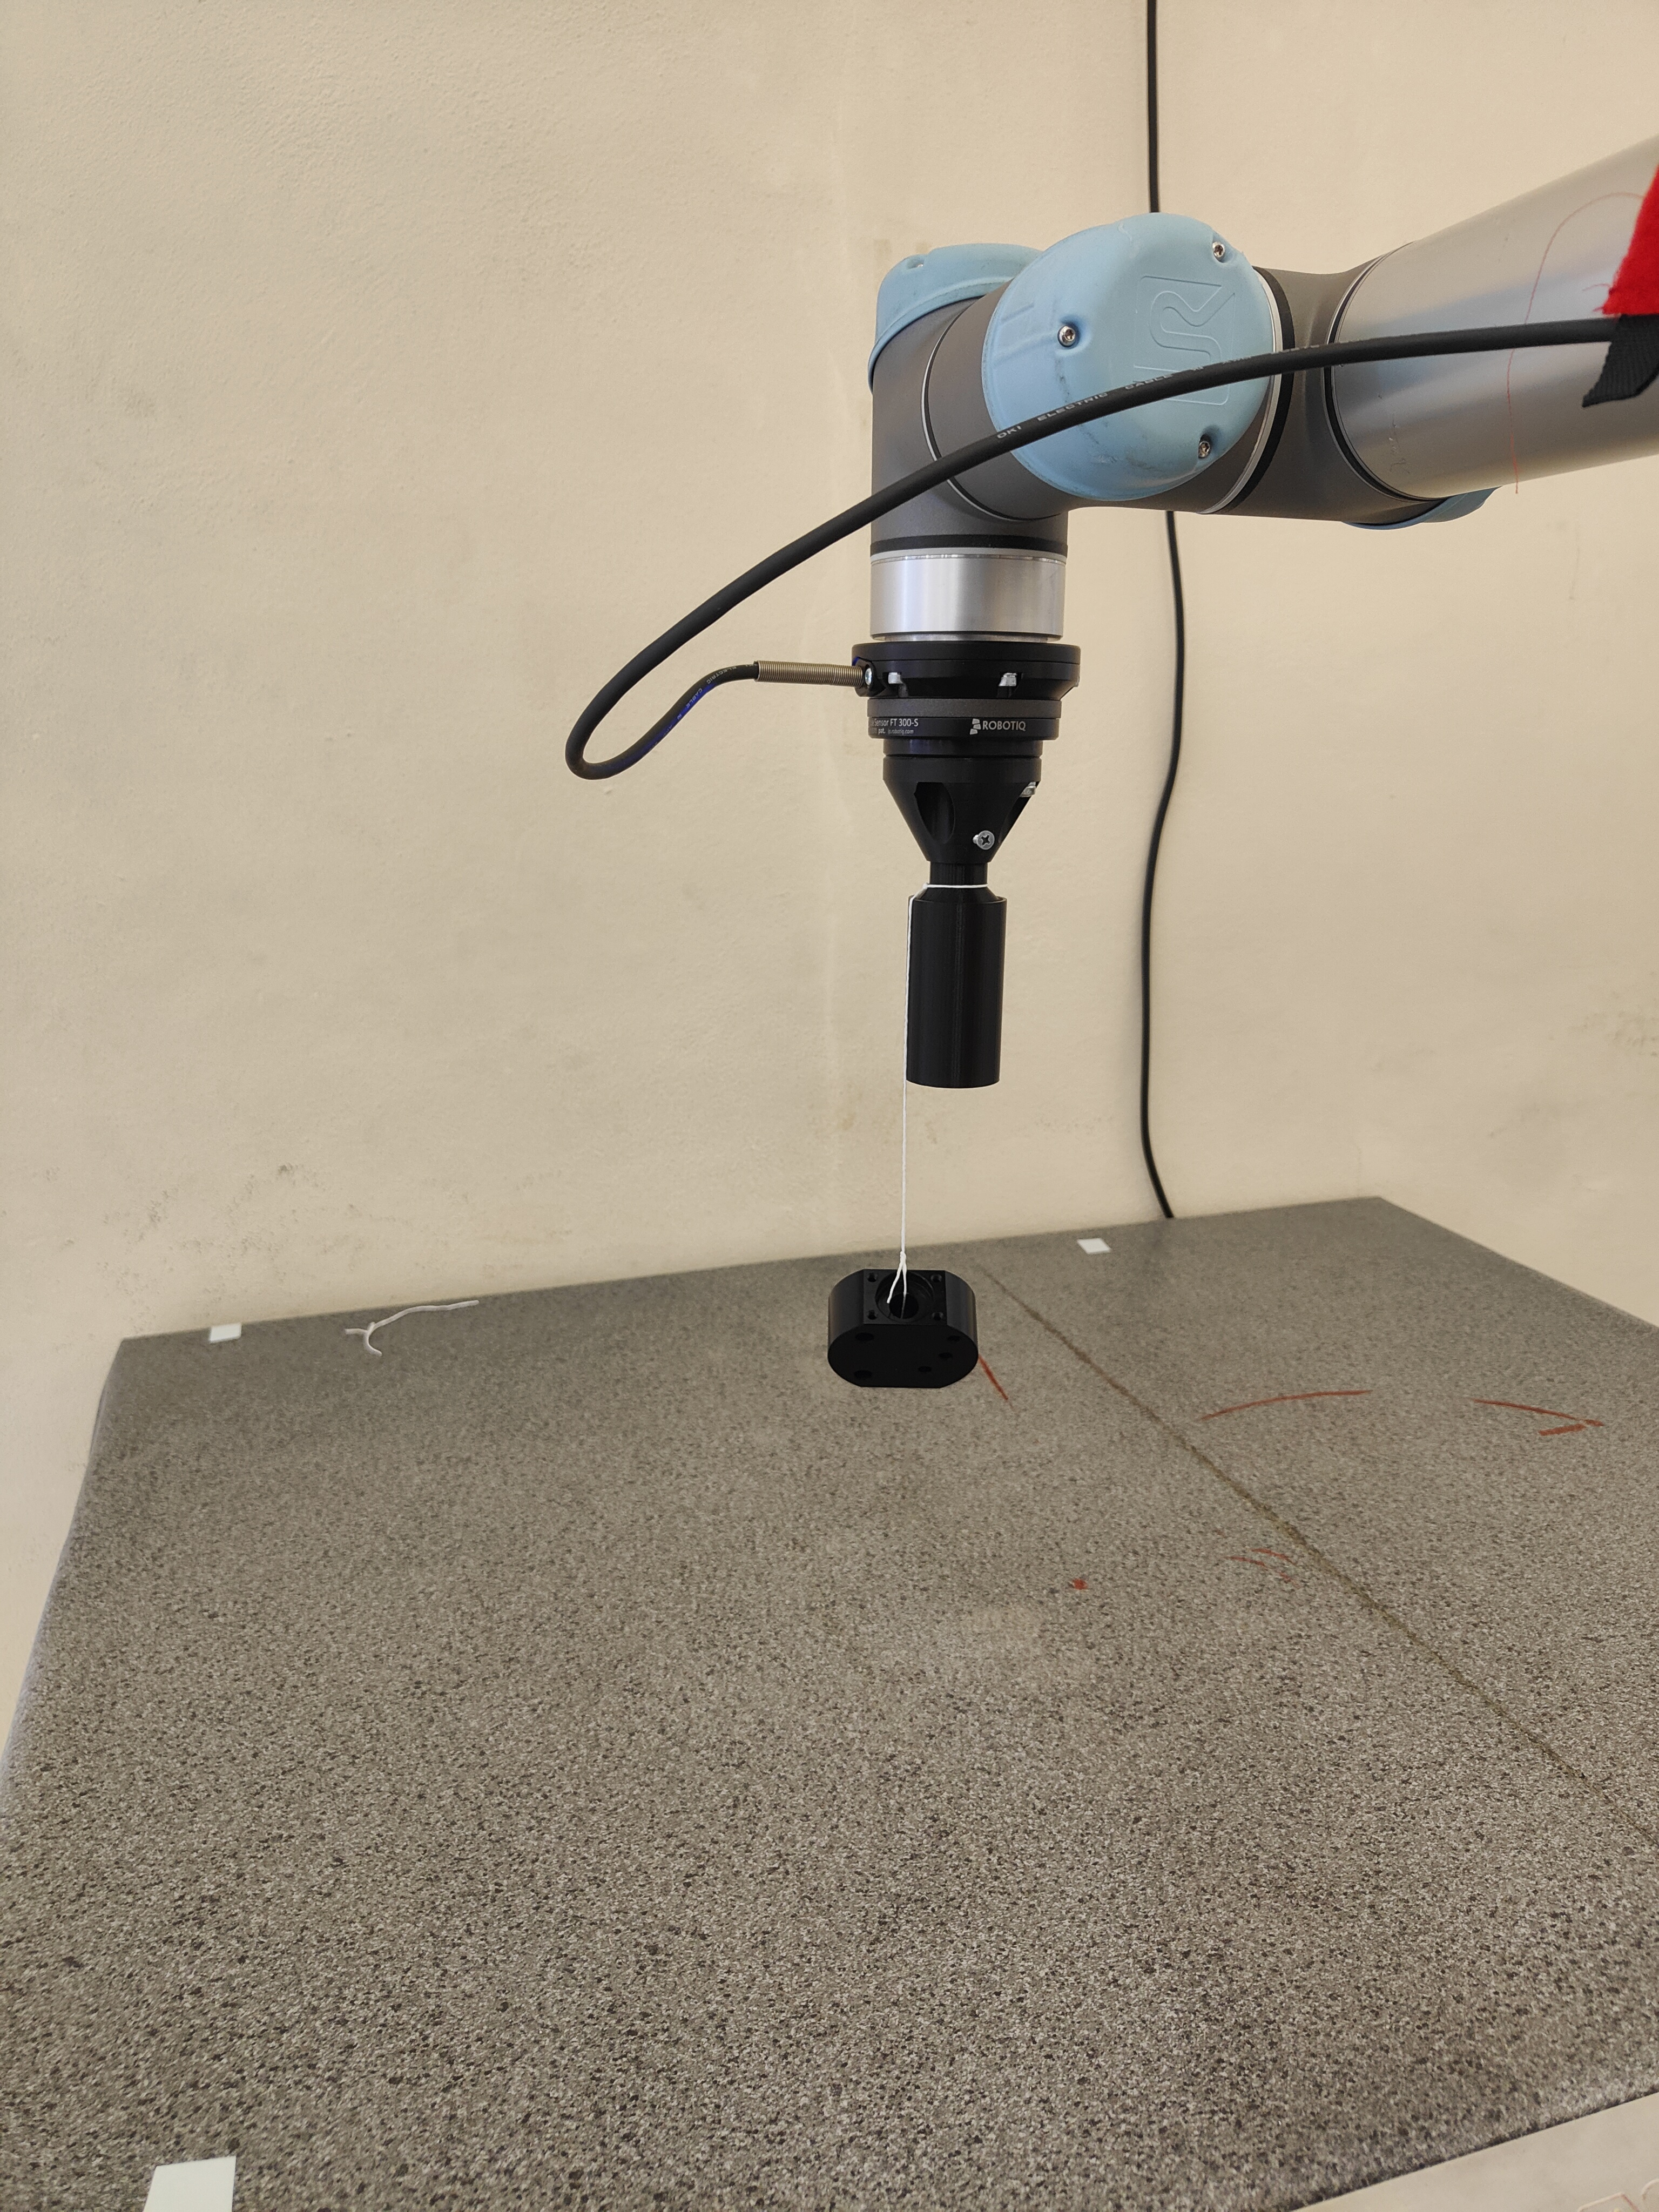
\includegraphics[width=\textwidth]{images/setup_z.jpg}
        \label{fig:setup}
    \end{subfigure}
    \caption{Setup esperimento (asse z)}\label{fig:setup_z}
\end{figure}
Dopo aver azzerato il sensore, per verificarne la reattivit\'{a}, il filo \'{e} stato tagliato di netto. 
Il taglio del filo \'{e} un ottimo modo per `simulare' un cambiamento di forza istantaneo.
\begin{figure}[H]
    \centering
    \includegraphics*[width=0.8\textwidth]{images/z_cut.png}
    \caption{Andamento taglio del filo lungo l'asse z}
    \label{fig:z_cut}
\end{figure}
In Figura \ref{fig:z_cut} viene mostrato l'andamento della forza rilevata dal sensore lungo l'asse z. 
Si pu\'{o} notare che, fino a quando il filo \'{e} attaccato al sensore, la forza rilevata \'{e} circa zero. 
Questo perch\'{e} il sensore \'{e} stato azzerato quando l'oggetto era gi\'{a} stato appeso. 
Nel momento in cui avviene il taglio, il grafico si allinea istantaneamente al peso reale dell'oggetto, 
ossia circa 1.5N.
Tale esperimento \'{e} stato ripetuto anche per gli altri due assi, come mostrato in Figura \ref{fig:setup_x}.
\begin{figure}[H]
    \centering
    \includegraphics*[width=0.45\textwidth]{images/setup_x.jpg}
    \caption{Setup esperimento (asse x)}
    \label{fig:setup_x}
\end{figure}
In questo modo la forza peso dell'oggetto grava univocamente sull'asse x. Ruotando l'end effector di 90° si ottiene il setup 
equivalente per l'asse y.
I risultati vengono mostrati in Figura \ref{fig:x_cut} e \ref{fig:y_cut}. 
\begin{figure}[H]
    \centering
    \includegraphics*[width=0.8\textwidth]{images/x_cut.png}
    \caption{Andamento taglio del filo lungo l'asse x}
    \label{fig:x_cut}
\end{figure}
\begin{figure}[H]
    \centering
    \includegraphics*[width=0.8\textwidth]{images/y_cut.png}
    \caption{Andamento taglio del filo lungo l'asse y}
    \label{fig:y_cut}
\end{figure}
A differenza di quanto riportato nei primi due grafici, l'andamento della forza rilevata lungo l'asse y, presenta un picco 
anomalo dovuto al taglio non sufficientemente netto del filo.
